% Provenance (never printed): see sources/outline_sources.md (Year 2: index minerals and zones,
% geothermometers and geobarometers, prograde and retrograde paths, metamorphic series,
% ultrahigh-pressure rocks and exhumation, ocean-floor metamorphism). Garnet-biotite
% calibration refitted from the Ferry and Spear (1978) brackets tabulated by Holdaway et al.
% (1997); GASP from Koziol and Newton (1988); thickening model after England and Thompson
% (1984) in figdata/bachelor-2/ptpaths.py; exercise and problem values in the Book 4 scratch
% calculators calc/ch11.py and calc/ch11b.py.
\chapter{Termobarometria e trajetórias P--T--t}\label{ch:b2:pt-paths}

Uma granada de alguns milímetros, crescida em um xisto, guarda em seu núcleo a composição
que tinha quando começou a crescer e em sua borda a composição que tinha quando parou. Cada
zona estava em equilíbrio com a biotita e o plagioclásio ao seu redor naquele momento, e a
maneira como o ferro, o magnésio e o cálcio se repartiam entre esses minerais depende da temperatura
e da pressão. Lida com a termodinâmica do capítulo anterior, uma granada diz a que
profundidade sua rocha foi soterrada e quão quente ficou; datada, diz quando, e com que rapidez a
rocha voltou a subir. Este capítulo transforma os minerais metamórficos em termômetros, barômetros
e relógios, e segue uma rocha ao longo de sua trajetória através da crosta.

\begin{recall}
\textbf{Do volume do ensino médio}: grau metamórfico, minerais-índice e isógradas.
\textbf{Do volume do primeiro ano}: a geoterma e a produção de calor radiogênico; a
crosta continental com cerca de \qty{35}{km} de espessura; a datação radiométrica, a temperatura de fechamento
de um mineral e a idade de resfriamento que ela fornece; a crosta oceânica e seu \omterm{def:b2:mantle-melting:peridotites}{peridotito}.
\textbf{Dos livros de física}: a equação do calor $\partial T/\partial t = \kappa\,
\partial^2 T/\partial z^2$ e a difusividade térmica $\kappa$. \textbf{Dos livros de
química}: a constante de equilíbrio, $\Delta_r G^\circ + RT\ln K = 0$, e as atividades em
soluções ideais. \textbf{Do \cref{ch:b2:metamorphic-facies}}: as \omterm{def:b2:metamorphic-facies:reaction}{reações metamórficas},
a \omterm{def:b2:metamorphic-facies:clapeyron}{inclinação de Clapeyron}, o diagrama \ce{Al2SiO5} e as fácies.
\end{recall}
% ledger: prem:moho-average

\section{As zonas metamórficas}\label{sec:b2:pt-paths:zones}

Nos lamitos das Terras Altas da Escócia, George Barrow mapeou na década de 1890 uma sequência de
zonas, cada uma marcada pelo primeiro aparecimento de um novo mineral-índice. Em direção ao grau
mais alto, à clorita se juntam sucessivamente a biotita, a granada, a estaurolita, a cianita e a silimanita;
nas seções-tipo, as zonas da granada à silimanita se formaram a cerca de 500 a
\qty{650}{\celsius} e 5 a \qty{7}{kbar}.
% ledger: iugs:barrow, barrow1893:paper, earle:regional

\begin{definition}[Zonas barrovianas; gradiente metamórfico de campo]\label{def:b2:pt-paths:barrovian}
As \emph{zonas barrovianas}\index{zonas barrovianas} são as zonas metamórficas dos
\omterm{def:b2:metamorphic-facies:protoliths}{metapelitos} na ordem clorita, biotita, granada, estaurolita, cianita, silimanita,
cada uma começando na isógrada de seu mineral-índice. O \emph{gradiente metamórfico de
campo}\index{gradiente metamórfico de campo} de uma região é a curva, no
plano pressão--temperatura, que passa pelas condições de pico registradas por suas rochas nos
lugares onde elas afloram hoje.
\end{definition}

Cada ponto de um gradiente de campo vem de uma rocha diferente, e cada rocha atingiu seu próprio
pico em seu próprio momento: o gradiente de campo não é a geoterma de nenhum instante, nem a
trajetória de nenhuma rocha. É o traço que os picos deixam na superfície de erosão atual.

\begin{omfigure}
\centering
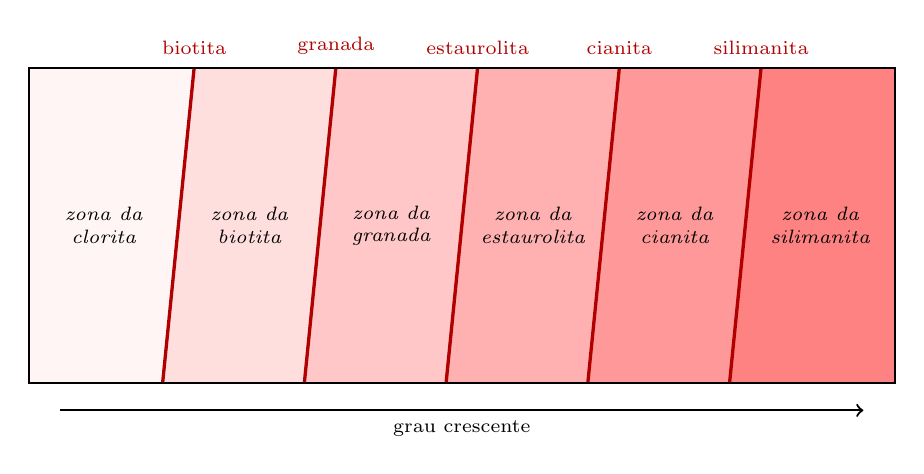
\begin{tikzpicture}[x=1cm, y=1cm]
\def\iso{{0,1.9,3.7,5.5,7.3,9.1,11}}
\foreach \i [evaluate=\i as \op using 4+9*\i] in {0,...,5} {
  \pgfmathsetmacro{\xa}{\iso[\i]}\pgfmathsetmacro{\xb}{\iso[\i+1]}
  \pgfmathsetmacro{\da}{(\i>0)*0.2}\pgfmathsetmacro{\db}{(\i<5)*0.2}
  \fill[red!\op!white] (\xa-\da,0) -- (\xb-\db,0) -- (\xb+\db,4) -- (\xa+\da,4) -- cycle;
}
\foreach \x/\n in {1.9/biotita, 3.7/granada, 5.5/estaurolita, 7.3/cianita, 9.1/silimanita} {
  \draw[very thick, red!70!black] (\x-0.2,0) -- (\x+0.2,4);
  \node[font=\scriptsize, red!70!black, anchor=south] at (\x+0.2,4.05) {\n};
}
\draw[thick] (0,0) rectangle (11,4);
\foreach \x/\z in {0.95/clorita, 2.8/biotita, 4.6/granada, 6.4/estaurolita, 8.2/cianita, 10.05/silimanita}
  \node[font=\scriptsize\itshape, align=center] at (\x,2) {zona da\\\z};
\draw[->, thick] (0.4,-0.35) -- node[below, font=\scriptsize] {grau crescente} (10.6,-0.35);
\end{tikzpicture}
\par\smallskip{\small \omterm{def:b2:pt-paths:barrovian}{Zonas barrovianas} em um mapa, esquemático. Cada isógrada (linha vermelha, nomeada
acima do mapa) é a linha onde seu mineral-índice aparece pela primeira vez; o grau, e a intensidade
do sombreado, aumentam para a direita. Cada zona leva o nome do mineral que aparece em seu
limite de baixo grau.}
\end{omfigure}
% ledger: iugs:barrow

As isógradas são mapeadas a partir dos aparecimentos de minerais, e só se tornam condições de pressão e de
temperatura quando as reações por trás delas são conhecidas. Para ir além, é preciso medir
a temperatura e a pressão em uma única rocha.

\section{Termômetros e barômetros}\label{sec:b2:pt-paths:thermobarometry}

\begin{definition}[Geotermômetro; geobarômetro; reação de troca; reação de transferência líquida]\label{def:b2:pt-paths:thermobarometry}
Um \emph{geotermômetro}\index{geotermômetro} (\emph{geobarômetro}\index{geobarômetro}) é
um equilíbrio entre minerais cuja posição depende sobretudo da temperatura (da pressão), de modo
que as composições dos minerais dão a temperatura (a pressão) de seu último
equilíbrio. Uma \emph{reação de troca}\index{reação de troca} permuta dois elementos
entre dois minerais, como o ferro e o magnésio entre granada e biotita, sem
criar nem destruir nenhum dos dois minerais. Uma \emph{reação de transferência líquida}\index{reação de transferência líquida}
produz certos minerais à custa de outros.
\end{definition}

O termômetro mais usado dos \omterm{def:b2:metamorphic-facies:protoliths}{metapelitos} é a troca de ferro e magnésio
entre granada e biotita,
\[
\ce{Fe3Al2Si3O12 + KMg3AlSi3O10(OH)2 <=> Mg3Al2Si3O12 + KFe3AlSi3O10(OH)2},
\]
almandina mais flogopita dando piropo mais anita. Sejam $X_{\text{Mg}}$ e $X_{\text{Fe}}$
as frações dos sítios ocupadas pelo magnésio e pelo ferro em cada mineral, e
\[
K_D = \frac{(X_{\text{Mg}}/X_{\text{Fe}})_{\text{granada}}}{(X_{\text{Mg}}/X_{\text{Fe}})_{\text{biotita}}}.
\]
% ledger: h97:fs-reaction

\begin{proposition}[Um equilíbrio de troca]\label{prop:b2:pt-paths:exchange}
Se a granada e a biotita são soluções ideais e $\Delta_r H$, $\Delta_r S$ e $\Delta_r V$ da
reação acima são constantes, então no equilíbrio
\[
3RT\ln K_D = -(\Delta_r H + P\,\Delta_r V) + T\,\Delta_r S,
\qquad\text{logo}\qquad
T = \frac{\Delta_r H + P\,\Delta_r V}{\Delta_r S - 3R\ln K_D}.
\]
\end{proposition}

\begin{proof}
Cada mineral tem três sítios para o ferro ou o magnésio. Em uma solução ideal, a atividade de
um membro extremo é o produto das frações de seus sítios que ele ocupa: $a_{\text{piropo}} =
X_{\text{Mg}}^3$ na granada, e assim por diante. A constante de equilíbrio é portanto
\[
K = \frac{a_{\text{piropo}}\,a_{\text{anita}}}{a_{\text{almandina}}\,a_{\text{flogopita}}}
= \frac{X_{\text{Mg,grt}}^3\,X_{\text{Fe,bt}}^3}{X_{\text{Fe,grt}}^3\,X_{\text{Mg,bt}}^3} = K_D^3 .
\]
No equilíbrio, $\Delta_r G^\circ(T, P) + RT\ln K = 0$, com $\Delta_r G^\circ = \Delta_r H -
T\,\Delta_r S + P\,\Delta_r V$ (o 1 de $P - 1$ desprezado), o que dá a primeira equação;
resolvendo-a em $T$, obtém-se a segunda.
\end{proof}

As constantes vêm de experimentos em que granada e biotita sintéticas trocaram ferro
e magnésio a temperatura conhecida e a \qty{2.07}{kbar}. Doze desses intervalos, de 550 a
\qty{800}{\celsius}, representados como $\ln K_D$ em função de $1/T$, ficam perto de uma reta (a figura
abaixo); ajustados por mínimos quadrados com $\Delta_r V = \qty{0.311}{J.bar^{-1}}$, eles dão
$\Delta_r H = \qty{52630}{J}$ e $\Delta_r S = \qty{20.19}{J.K^{-1}}$, os valores de
recálculos publicados dos mesmos dados. A temperatura mais alta, a razão $K_D$ sobe
em direção a 1: a granada toma uma parte maior do magnésio.
% ledger: h97:fs-data, h97:ideal, h97:fs-reaction

\begin{omfigure}
\centering
\begin{tikzpicture}
\begin{axis}[omrecord, width=0.62\linewidth, height=5.2cm,
  xmin=0.9, xmax=1.25, ymin=-1.9, ymax=-1.1,
  xlabel={$1000/T$ (\unit{K^{-1}})}, ylabel={$\ln K_D$},
  tick label style={font=\scriptsize}, label style={font=\small},
  x tick label style={/pgf/number format/.cd, fixed, precision=2}]
\addplot[only marks, mark=*, mark size=1.6pt, blue!70!black]
  table[x expr={1000/(\thisrow{T_C}+273.15)}, y=lnKD] {figdata/out/bachelor-2-ptpaths-fs.dat};
\addplot[thick, red!75!black, domain=0.9:1.25, samples=2] {(-52630-2070*0.311)/(3*8.31441)*x/1000 + 20.19/(3*8.31441)};
\end{axis}
\end{tikzpicture}
\par\smallskip{\small Troca granada--biotita: os doze intervalos experimentais a
\qty{2.07}{kbar} (azul, tal como tabelados por Holdaway e coautores, 1997) e a reta da
proposição com os $\Delta_r H$ e $\Delta_r S$ ajustados (vermelho).}
\end{omfigure}
% ledger: h97:fs-data, h97:ideal

Para $K_D = 0.18$ a \qty{5}{kbar}, $T = (52630 + 0.311\times5000)/(20.19 - 3\times8.314
\times\ln 0.18) = 54185/62.96 = \qty{861}{K}$, ou \qty{587}{\celsius}. Um quilobar a mais
acrescenta $0.311\times1000/62.96 = \qty{4.9}{K}$: a reação troca íons de mesma carga
entre sítios de tamanho quase igual, sua variação de volume é pequena, e a pressão quase não
importa. É isso que faz um termômetro.

Um barômetro precisa do contrário: uma reação com grande variação de volume. A \omterm{def:b2:pt-paths:thermobarometry}{reação de
transferência líquida}
\[
\ce{3 CaAl2Si2O8 <=> Ca3Al2Si3O12 + 2 Al2SiO5 + SiO2},
\]
anortita dando grossulária, cianita e quartzo, acomoda os átomos de três feldspatos em
minerais mais densos: $\Delta_r V = \qty{-6.21}{J.bar^{-1}}$, vinte vezes o da troca.
Seu equilíbrio entre membros extremos, revertido em experimentos a 900 a \qty{1250}{\celsius} e 19
a \qty{28}{kbar}, segue
\[
P_0 = 22.80\,T - 1093 \qquad (P_0 \text{ em bar}, T \text{ em } \unit{\celsius}).
\]
Em uma rocha, a grossulária é uma pequena parte da granada e a anortita uma parte do
plagioclásio. Com atividades ideais, $a_{\text{grossulária}} = X_{\text{Ca,grt}}^3$ e
$a_{\text{anortita}} = X_{\text{an}}$, a condição $\Delta_r G^\circ + RT\ln K = 0$
escrita em $P$ e em $P_0$ dá
\[
P = P_0 + \frac{RT}{6.21}\,\ln\frac{X_{\text{Ca,grt}}^3}{X_{\text{an}}^3}
\qquad (T \text{ em kelvin no segundo termo}).
\]
Esse \omterm{def:b2:pt-paths:thermobarometry}{geobarômetro}, chamado GASP a partir dos quatro minerais (granada, aluminossilicato, sílica,
plagioclásio), serve onde quer que um \omterm{def:b2:metamorphic-facies:protoliths}{metapelito} contenha os quatro.
% ledger: kn88:gasp, rh95:gb-gasp

\begin{method}[Temperatura e pressão de uma rocha]\label{met:b2:pt-paths:intersection}
(1) Meça, em minerais que cresceram juntos, as composições de que o termômetro e o
barômetro precisam. (2) Suponha uma pressão e calcule a temperatura com o termômetro.
(3) A essa temperatura, calcule a pressão com o barômetro. (4) Repita (2) e (3)
até que nenhuma das duas mude; duas ou três rodadas bastam, já que cada equação depende pouco
da variável que a outra fixa. Graficamente, a resposta está onde a linha do
termômetro cruza a linha do barômetro. (5) Propague as incertezas: para
erros independentes, $\sigma_T^2 = (\partial T/\partial\ln K_D)^2\sigma_{\ln K_D}^2 +
(\partial T/\partial P)^2\sigma_P^2$, e analogamente para $P$.
\end{method}

\begin{omfigure}
\centering
\begin{tikzpicture}
\begin{axis}[omrecord, width=0.78\linewidth, height=6.4cm,
  xmin=400, xmax=800, ymin=0, ymax=12, xlabel={$T$ (\unit{\celsius})}, ylabel={$P$ (\unit{kbar})},
  tick label style={font=\scriptsize}, label style={font=\small}, clip=false]
\addplot[thick, red!75!black] table[x=kd12, y=P_kbar] {figdata/out/bachelor-2-ptpaths-gb.dat};
\addplot[thick, red!75!black] table[x=kd15, y=P_kbar] {figdata/out/bachelor-2-ptpaths-gb.dat};
\addplot[thick, red!75!black] table[x=kd18, y=P_kbar] {figdata/out/bachelor-2-ptpaths-gb.dat};
\addplot[thick, red!75!black] table[x=kd21, y=P_kbar] {figdata/out/bachelor-2-ptpaths-gb.dat};
\addplot[thick, red!75!black] table[x=kd24, y=P_kbar] {figdata/out/bachelor-2-ptpaths-gb.dat};
\addplot[thick, blue!70!black] table[x=T_C, y=r15] {figdata/out/bachelor-2-ptpaths-gasp.dat};
\addplot[thick, blue!70!black] table[x=T_C, y=r20] {figdata/out/bachelor-2-ptpaths-gasp.dat};
\addplot[thick, blue!70!black] table[x=T_C, y=r25] {figdata/out/bachelor-2-ptpaths-gasp.dat};
\addplot[thick, blue!70!black] table[x=T_C, y=r30] {figdata/out/bachelor-2-ptpaths-gasp.dat};
\node[font=\tiny, red!75!black, anchor=west] at (axis cs:452,0.5) {0.12};
\node[font=\tiny, red!75!black, anchor=west] at (axis cs:511,0.5) {0.15};
\node[font=\tiny, red!75!black, anchor=west] at (axis cs:568,0.5) {0.18};
\node[font=\tiny, red!75!black, anchor=west] at (axis cs:622,0.5) {0.21};
\node[font=\tiny, red!75!black, anchor=west] at (axis cs:675,0.5) {0.24};
\node[font=\tiny, blue!70!black, anchor=west] at (axis cs:802,8.97) {0.15};
\node[font=\tiny, blue!70!black, anchor=west] at (axis cs:802,10.21) {0.20};
\node[font=\tiny, blue!70!black, anchor=west] at (axis cs:802,11.17) {0.25};
\node[font=\tiny, blue!70!black, anchor=west] at (axis cs:802,11.96) {0.30};
\end{axis}
\end{tikzpicture}
\par\smallskip{\small Isotermas granada--biotita (vermelho, íngremes, rotuladas com $K_D$) e isóbaras
GASP (azul, rotuladas à direita com a razão $X_{\text{Ca}}/X_{\text{an}}$ entre a
grossulária na granada e a anortita no plagioclásio), a partir das calibrações desta seção. Uma rocha que contém os dois pares fica
onde suas duas linhas se cruzam.}
\end{omfigure}
% ledger: h97:ideal, h97:fs-reaction, kn88:gasp

As linhas do termômetro são quase verticais, as do barômetro inclinadas: elas se cruzam segundo um
ângulo amplo, o que mantém a interseção precisa. A mistura ideal é a principal simplificação
deste capítulo. As granadas reais contêm cálcio e manganês, as biotitas reais alumínio,
titânio e ferro férrico, e as calibrações que os corrigem deslocam as temperaturas de
dezenas de graus (em uma região bem estudada, \qty{574}{\celsius} em vez de
\qty{530}{\celsius}); as melhores reivindicam uma incerteza de cerca de \qty{25}{\celsius}.
% ledger: h97:ideal, h97:corrections

\section{Trajetórias pressão--temperatura}\label{sec:b2:pt-paths:paths}

Uma rocha não atinge sua pressão máxima e sua temperatura máxima no mesmo momento.
Ela é soterrada e aquecida, depois trazida de volta e resfriada, e seus minerais reagem ao longo
de todo o caminho.

\begin{definition}[Trajetória P--T; trajetórias progressiva e retrógrada; condições do pico metamórfico]\label{def:b2:pt-paths:paths}
A \emph{trajetória P--T}\index{trajetória P--T} de uma rocha é a sequência de pressões e de
temperaturas pelas quais ela passou durante um evento metamórfico. Sua \emph{trajetória
progressiva}\index{trajetória progressiva} é a parte ao longo da qual a temperatura sobe, sua \emph{trajetória
retrógrada}\index{trajetória retrógrada} a parte ao longo da qual ela desce. As \emph{condições do pico
metamórfico}\index{condições do pico metamórfico} são a pressão e a temperatura na
temperatura mais alta da trajetória, o pico térmico; o pico de pressão, ou pico bárico, não
coincide necessariamente com ele.
\end{definition}
% ledger: scmr:ptt

Uma trajetória é \emph{horária} quando, desenhada com a temperatura para a direita e a pressão para cima,
o pico térmico vem depois do pico bárico, durante a descompressão; é
\emph{anti-horária} quando o pico térmico é atingido enquanto a pressão ainda sobe. Qual
sentido uma rocha segue depende de como o calor chegou até ela, e o caso mais simples pode ser
calculado.
% ledger: scmr:ptt

Imagine-se uma crosta de \qty{35}{km} de espessura, em regime estacionário, com uma produção de calor de
\qty{1.0}{\micro W.m^{-3}}, um fluxo de calor de \qty{25}{mW.m^{-2}} vindo de baixo, uma condutividade
de \qty{2.5}{W.m^{-1}.K^{-1}} e uma difusividade de \qty{1e-6}{m^2.s^{-1}}, as três últimas
dentro das faixas medidas em rochas. Seu fluxo de calor em superfície é de \qty{60}{mW.m^{-2}} e seu Moho fica a
\qty{595}{\celsius}. Uma colisão empilha uma segunda cópia dessa crosta sobre ela, depressa
em comparação com o tempo de que o calor precisa para se deslocar: as rochas da lâmina inferior conservam suas
temperaturas, mas ficam \qty{35}{km} mais fundas, de modo que a geoterma se torna um dente de serra, com
rochas a \qty{0}{\celsius} a \qty{35}{km} sob rochas quentes da lâmina superior. A crosta tem
agora \qty{70}{km} de espessura e contém o dobro de rocha produtora de calor. Trinta milhões de anos depois
do empilhamento, a erosão começa e remove \qty{35}{km} em 70 milhões de anos
(\qty{0.5}{mm.yr^{-1}}).
% ledger: delaney:conductivity, roy:granitic-k, vila:heat-production, prem:moho-average, et84:ptt

\begin{proposition}[Escala de tempo do relaxamento térmico]\label{prop:b2:pt-paths:relaxation}
Em uma camada de espessura $L$ cujas duas faces são mantidas a temperatura fixa, uma perturbação
de temperatura da forma $\sin(\pi z/L)$ decai como $e^{-t/\tau}$, com
\[
\tau = \frac{L^2}{\pi^2\kappa}.
\]
\end{proposition}

\begin{proof}
Escreva-se $\theta(z, t) = f(t)\sin(\pi z/L)$, que se anula em $z = 0$ e $z = L$. A equação
do calor $\partial\theta/\partial t = \kappa\,\partial^2\theta/\partial z^2$ dá
$f'\sin(\pi z/L) = -\kappa(\pi/L)^2 f\sin(\pi z/L)$, logo $f' = -f/\tau$ com $\tau =
L^2/(\pi^2\kappa)$, e $f = f(0)\,e^{-t/\tau}$.
\end{proof}

O dente de serra tem um comprimento de onda da ordem da espessura de uma lâmina: com $L =
\qty{35}{km}$, $\tau = \qty{3.9}{Myr}$, e a cunha fria a \qty{35}{km} se apaga em
dez milhões de anos. A crosta espessada inteira, $L = \qty{70}{km}$, relaxa em $\tau =
\qty{16}{Myr}$, de modo que o aquecimento continua por dezenas de milhões de anos, em direção à geoterma muito
mais quente que sustenta uma crosta duas vezes mais espessa e com o dobro de rocha produtora de calor.
A figura
abaixo mostra as geotermas calculadas.
% ledger: delaney:conductivity

\begin{omfigure}
\centering
\begin{tikzpicture}
\begin{axis}[omrecord, width=0.62\linewidth, height=6.6cm,
  xmin=0, xmax=1000, ymin=0, ymax=80, y dir=reverse,
  xlabel={$T$ (\unit{\celsius})}, ylabel={profundidade (\unit{km})},
  legend style={font=\scriptsize, at={(0.02,0.02)}, anchor=south west},
  tick label style={font=\scriptsize}, label style={font=\small}]
\addplot[thick, black] table[x=t0, y=z_km] {figdata/out/bachelor-2-ptpaths-geo.dat};
\addlegendentry{\qty{0}{Myr}}
\addplot[thick, blue!70!black] table[x=t10, y=z_km] {figdata/out/bachelor-2-ptpaths-geo.dat};
\addlegendentry{\qty{10}{Myr}}
\addplot[thick, orange!85!black] table[x=t30, y=z_km] {figdata/out/bachelor-2-ptpaths-geo.dat};
\addlegendentry{\qty{30}{Myr}}
\addplot[thick, red!75!black] table[x=t60, y=z_km] {figdata/out/bachelor-2-ptpaths-geo.dat};
\addlegendentry{\qty{60}{Myr}}
\end{axis}
\end{tikzpicture}
\par\smallskip{\small Geotermas depois da duplicação por empilhamento de uma crosta de \qty{35}{km}, calculadas
com a equação do calor (profundidades sob a superfície do momento; a erosão começa a
\qty{30}{Myr}). Preto: o dente de serra logo depois do empilhamento. A base da crosta espessada,
a \qty{595}{\celsius} no início, passa de \qty{900}{\celsius} depois de 60 milhões de anos.}
\end{omfigure}
% ledger: et84:ptt

Siga-se a rocha que estava na superfície antes do empilhamento e fica a \qty{35}{km} logo
depois dele, sob \qty{9.6}{kbar}. Em cinco milhões de anos, ela se aquece de 0 a
\qty{395}{\celsius} sem se mover; no início da erosão, já chegou a
\qty{558}{\celsius}. A erosão então a faz subir, mas o calor continua chegando mais depressa do que
escapa: a rocha ainda se aquece quando já subiu \qty{6}{km}, e atinge seu pico
térmico, \qty{593}{\celsius} a \qty{7.8}{kbar}, 43 milhões de anos depois do empilhamento. Só
então ela se resfria, passando por \qty{405}{\celsius} a \qty{13}{km} de profundidade e
\qty{74}{Myr}, a caminho da superfície. A trajetória (a figura abaixo) é horária. Ela também
permanece a menos de \qty{50}{\celsius} de sua temperatura de pico durante trinta milhões de anos, cerca de um
terço de toda a sua viagem, como England e Thompson constataram em 1984 para a maioria dos casos
geologicamente plausíveis: uma rocha passa muito tempo perto de seu pico, e os minerais que ela conserva
registram sobretudo essa etapa.
% ledger: et84:ptt

\begin{omfigure}
\centering
\begin{tikzpicture}
\begin{axis}[omrecord, width=0.78\linewidth, height=6.2cm,
  xmin=0, xmax=800, ymin=0, ymax=11, xlabel={$T$ (\unit{\celsius})}, ylabel={$P$ (\unit{kbar})},
  tick label style={font=\scriptsize}, label style={font=\small}]
\addplot[thick, gray, densely dashed, restrict x to domain=0:504] table[x=T_C, y=P_kbar] {figdata/out/bachelor-2-facies-hm93-kyand.dat};
\addplot[thick, gray, densely dashed] table[x=T_C, y=P_kbar] {figdata/out/bachelor-2-facies-hm93-kysil.dat};
\addplot[thick, gray, densely dashed] table[x=T_C, y=P_kbar] {figdata/out/bachelor-2-facies-hm93-andsil.dat};
\addplot[very thick, red!75!black, postaction={decorate}, decoration={markings,
  mark=at position 0.2 with {\arrow{Stealth[length=2.5mm]}},
  mark=at position 0.52 with {\arrow{Stealth[length=2.5mm]}},
  mark=at position 0.8 with {\arrow{Stealth[length=2.5mm]}}}] table[x=T_C, y=P_kbar] {figdata/out/bachelor-2-ptpaths-path.dat};
\node[font=\scriptsize\bfseries, gray] at (axis cs:330,6.5) {cianita};
\node[font=\scriptsize\bfseries, gray] at (axis cs:520,1.0) {andaluzita};
\node[font=\scriptsize\bfseries, gray] at (axis cs:740,4.0) {silimanita};
\node[font=\scriptsize, red!75!black, anchor=south] at (axis cs:200,9.7) {aquecimento em profundidade};
\node[font=\scriptsize, red!75!black, anchor=west] at (axis cs:603,8.9) {pico térmico};
\node[font=\scriptsize, red!75!black, anchor=west] at (axis cs:110,2.7) {subida com resfriamento};
\end{axis}
\end{tikzpicture}
\par\smallskip{\small \omterm{def:b2:pt-paths:paths}{Trajetória P--T} da rocha que fica a \qty{35}{km} logo depois do
empilhamento (vermelho, amostrada a cada dois milhões de anos), calculada com o modelo das geotermas acima,
sobre o diagrama experimental \ce{Al2SiO5} do \cref{ch:b2:metamorphic-facies} (cinza). O
pico de pressão vem primeiro, o pico térmico durante a descompressão: uma trajetória horária, que
nunca sai do campo da cianita.}
\end{omfigure}
% ledger: et84:ptt, hm93:table11

O modelo mostra também por que algumas trajetórias giram no outro sentido. O espessamento sozinho só aquece uma rocha
depois que ela foi soterrada, de modo que seu pico térmico vem durante a \omterm{def:b2:pt-paths:exhumation}{exumação}. Uma rocha cuja
temperatura sobe enquanto ainda está sendo soterrada precisa de calor de outra origem, como um \omterm{def:b2:magma-emplacement:magma}{magma}
que sobe na crosta acima ou ao lado dela, e segue uma trajetória anti-horária. E, na
crosta espessada, a base se aquece muito acima de sua temperatura inicial: England e Thompson
concluíram que uma fusão considerável da crosta é uma consequência provável do espessamento,
o assunto do \cref{ch:b2:crustal-melting}.
% ledger: et84:ptt, scmr:ptt

\section{Acrescentar o tempo}\label{sec:b2:pt-paths:time}

\begin{definition}[Trajetória P--T--t]\label{def:b2:pt-paths:ptt}
A \emph{trajetória P--T--t}\index{trajetória P--T--t} de uma rocha é sua \omterm{def:b2:pt-paths:paths}{trajetória P--T} com o momento
em que cada ponto foi atingido.
\end{definition}
% ledger: scmr:ptt

O tempo vem da datação radiométrica. Um mineral que cresceu durante o evento e conservou
seus isótopos-filhos desde então, como uma zona de granada datada pelo
método samário--neodímio, data seu próprio crescimento, e sua
composição dá a pressão e a temperatura desse momento. Um mineral que cresceu
antes, a temperatura mais alta, dá em vez disso uma idade de resfriamento: o momento em que a rocha
se resfriou abaixo da temperatura de fechamento daquele mineral e daquele sistema isotópico (volume do primeiro
ano). Para o argônio em um grão de muscovita de \qty{100}{\micro m} de raio, resfriando-se a
\qty{10}{\celsius} por milhão de anos, a temperatura de fechamento é de \qty{405}{\celsius} a
\qty{5}{kbar} e de \qty{425}{\celsius} a \qty{10}{kbar}.
% ledger: h09:muscovite

\begin{definition}[Exumação; taxa de exumação]\label{def:b2:pt-paths:exhumation}
A \emph{exumação}\index{exumação} é o movimento de uma rocha em direção à superfície da Terra,
pela remoção das rochas acima dela. A \emph{taxa de exumação}\index{taxa de exumação} é a
taxa de diminuição de sua profundidade.
\end{definition}

\begin{proposition}[Taxas a partir de dois pontos datados]\label{prop:b2:pt-paths:rates}
Se uma rocha estava à temperatura $T_1$ e à profundidade $z_1$ no tempo $t_1$ e a $T_2$, $z_2$ em um
tempo posterior $t_2$ (idades contadas para trás a partir de hoje, $t_1 > t_2$), suas taxas médias de resfriamento e de
\omterm{def:b2:pt-paths:exhumation}{exumação} no intervalo são
\[
\frac{T_1 - T_2}{t_1 - t_2}
\qquad\text{e}\qquad
\frac{z_1 - z_2}{t_1 - t_2},
\]
e suas incertezas, para erros independentes nas duas idades, decorrem de
$\sigma_{t_1 - t_2}^2 = \sigma_{t_1}^2 + \sigma_{t_2}^2$.
\end{proposition}

\begin{proof}
Uma taxa média é uma diferença dividida pelo tempo decorrido $t_1 - t_2$; a variância de uma
diferença de grandezas independentes é a soma de suas variâncias.
\end{proof}

A profundidade em que uma idade de resfriamento foi fixada raramente é medida: ela é estimada a partir da
geoterma da época, e é por isso que as \omterm{def:b2:pt-paths:exhumation}{taxas de exumação} são menos certas que as taxas de resfriamento.
Uma pressão, quando uma \omterm{def:b2:metamorphic-facies:assemblage}{assembleia mineral} fornece uma, fixa diretamente a profundidade, como
$z = P/(\bar\rho g)$, com $\bar\rho$ a densidade média das rochas acima.

\section{Séries metamórficas e cinturões pareados}\label{sec:b2:pt-paths:series}

\begin{definition}[Série metamórfica; cinturões metamórficos pareados]\label{def:b2:pt-paths:series}
Uma \emph{série metamórfica}\index{série metamórfica} (ou série de fácies) é uma sequência de
\omterm{def:b2:metamorphic-facies:facies}{fácies metamórficas} desenvolvidas sob a mesma faixa de razões entre pressão e temperatura,
e que ocupa portanto um setor radial do plano pressão--temperatura.
Os \emph{cinturões metamórficos pareados}\index{cinturões metamórficos pareados} são dois cinturões paralelos de
mesma idade, um de série de alta pressão e outro de série de baixa pressão.
\end{definition}
% ledger: scmr:ptt, wallis24:paired

Três séries são comumente distinguidas. Uma razão alta entre pressão e temperatura, ao longo de um
gradiente frio, leva da fácies zeólita aos xistos azuis e eclogitos: a série
das zonas de subducção. Uma razão intermediária leva pelas fácies xisto verde, anfibolito e
granulito, com cianita e depois silimanita nos \omterm{def:b2:metamorphic-facies:protoliths}{metapelitos}: a série barroviana. Uma razão
baixa, ao longo de gradientes quentes como os que há perto das intrusões, produz andaluzita e depois
silimanita: a série de baixa pressão, ou série de Buchan. A figura abaixo traça três gradientes
através do diagrama dos aluminossilicatos.
% ledger: scmr:ptt, scmr:facies, iugs:barrow, fub:paired

\begin{omfigure}
\centering
\begin{tikzpicture}
\begin{axis}[omrecord, width=0.78\linewidth, height=6.2cm,
  xmin=0, xmax=900, ymin=0, ymax=12, xlabel={$T$ (\unit{\celsius})}, ylabel={$P$ (\unit{kbar})},
  tick label style={font=\scriptsize}, label style={font=\small}]
\addplot[thick, gray, densely dashed, restrict x to domain=0:504] table[x=T_C, y=P_kbar] {figdata/out/bachelor-2-facies-hm93-kyand.dat};
\addplot[thick, gray, densely dashed] table[x=T_C, y=P_kbar] {figdata/out/bachelor-2-facies-hm93-kysil.dat};
\addplot[thick, gray, densely dashed] table[x=T_C, y=P_kbar] {figdata/out/bachelor-2-facies-hm93-andsil.dat};
\addplot[very thick, blue!70!black] table[x=T_C, y=g10] {figdata/out/bachelor-2-ptpaths-series.dat};
\addplot[very thick, green!45!black] table[x=T_C, y=g25] {figdata/out/bachelor-2-ptpaths-series.dat};
\addplot[very thick, orange!85!black] table[x=T_C, y=g60] {figdata/out/bachelor-2-ptpaths-series.dat};
\node[font=\scriptsize, blue!70!black, rotate=52, anchor=south] at (axis cs:330,8.5) {\qty{10}{\celsius\per\km}};
\node[font=\scriptsize, green!45!black, rotate=28, anchor=south] at (axis cs:640,7.0) {\qty{25}{\celsius\per\km}};
\node[font=\scriptsize, orange!85!black, rotate=12, anchor=south] at (axis cs:800,3.65) {\qty{60}{\celsius\per\km}};
\node[font=\scriptsize\bfseries, gray] at (axis cs:120,5.5) {cianita};
\node[font=\scriptsize\bfseries, gray] at (axis cs:470,1.1) {andaluzita};
\node[font=\scriptsize\bfseries, gray] at (axis cs:800,1.6) {silimanita};
\end{axis}
\end{tikzpicture}
\par\smallskip{\small Três gradientes geotérmicos a partir de uma superfície a \qty{10}{\celsius},
convertidos em pressão com uma densidade média de \qty{2800}{kg.m^{-3}}, sobre o diagrama experimental
\ce{Al2SiO5} (cinza). O gradiente frio permanece no campo da cianita, o
intermediário passa da cianita à silimanita, o quente atravessa o campo da andaluzita
antes de chegar à silimanita.}
\end{omfigure}
% ledger: hm93:table11

A ideia das séries veio do Japão, onde Akiho Miyashiro as definiu em 1961. No
sudoeste do país, o cinturão de Sanbagawa, de \omterm{def:b2:metamorphic-facies:metamorphism}{metamorfismo} de alta pressão e baixa temperatura,
estende-se por mais de \qty{800}{km} ao lado do cinturão de Ryoke, de \omterm{def:b2:metamorphic-facies:metamorphism}{metamorfismo} de alta temperatura e
baixa pressão, os dois separados por uma falha importante: o par clássico. O
cinturão de Sanbagawa é uma antiga zona de subducção, o cinturão de Ryoke o arco vulcânico acima dela. Uma
zona de subducção produz assim as duas séries ao mesmo tempo, rochas frias arrastadas para baixo pela placa
que afunda, rochas quentes aquecidas no arco; cinturões pareados do mesmo tipo são conhecidos em torno do
Pacífico.
% ledger: wallis24:paired, koguchi17:paired, fub:paired, scmr:ptt

\section{Ultra-alta pressão e exumação}\label{sec:b2:pt-paths:uhp}

Em 1984 foi descrito, no maciço de Dora Maira, nos Alpes Ocidentais, um quartzito
cujas granadas, de até \qty{25}{cm} e quase de piropo puro, englobam grãos de
coesita, o polimorfo denso da sílica, em parte retransformada em quartzo; a expansão
durante essa inversão fraturou radialmente a granada hospedeira em torno de cada grão. A coesita e
seus minerais companheiros implicam pelo menos \qty{28}{kbar} a cerca de \qty{700}{\celsius}: rochas da
crosta continental superior, antes sedimentos, tinham descido a \qty{90}{km} ou mais e
voltado.
% ledger: chopin84:coesite

\begin{definition}[Metamorfismo de ultra-alta pressão]\label{def:b2:pt-paths:uhp}
O \emph{metamorfismo de ultra-alta pressão}\index{metamorfismo de ultra-alta pressão} é o
\omterm{def:b2:metamorphic-facies:metamorphism}{metamorfismo} de rochas crustais a pressões altas o bastante para que cresça coesita, ou diamante.
\end{definition}

\begin{omfigure}
\centering
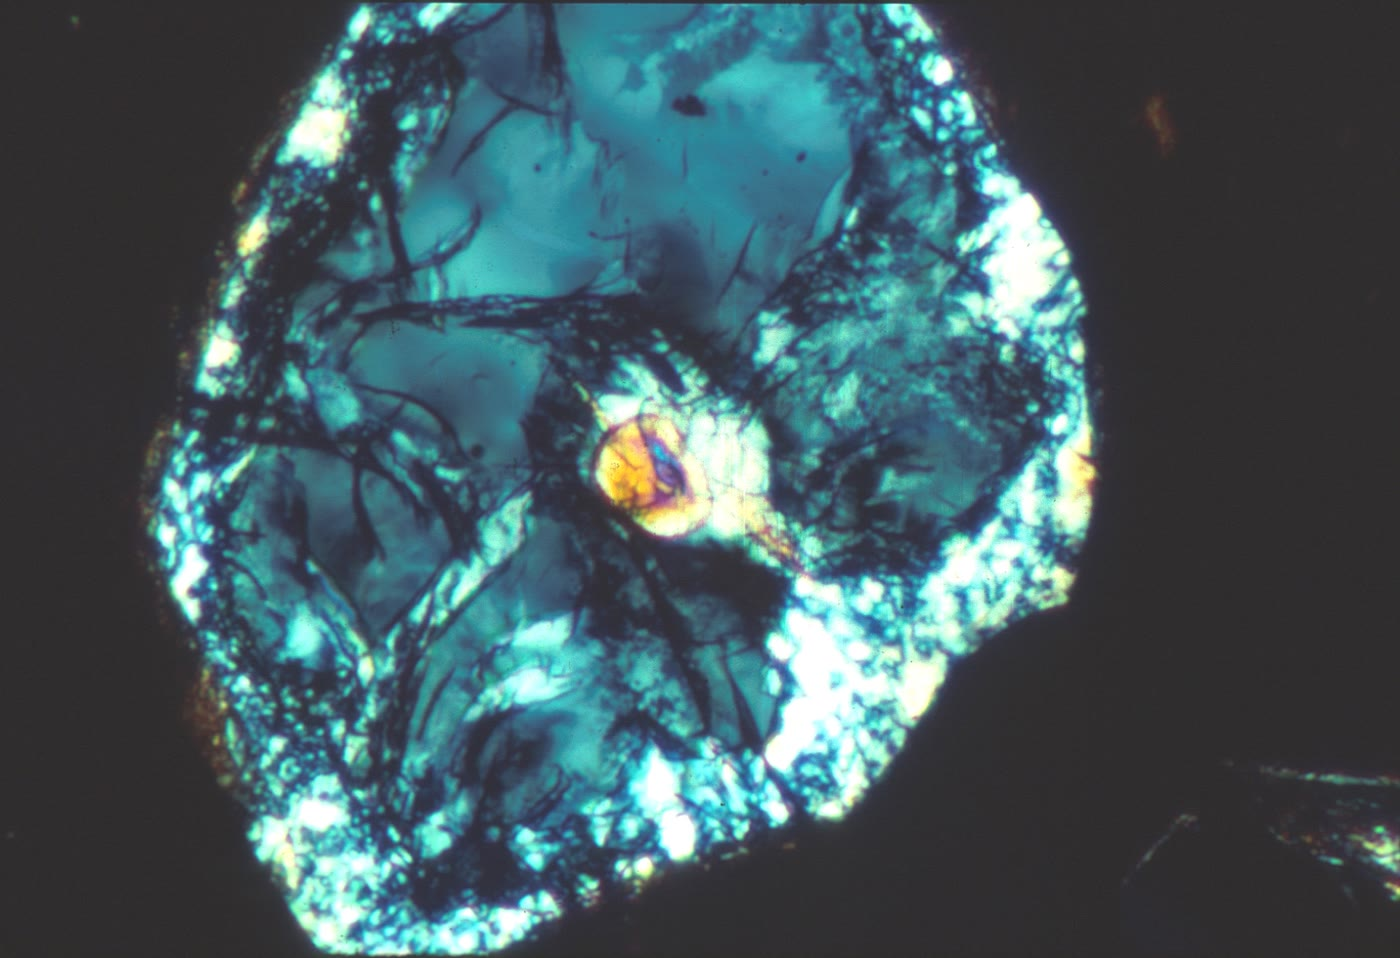
\includegraphics[width=0.62\linewidth]{images/book4/b2-11-coesite.jpg}
\par\smallskip{\small Coesita em um eclogito, com cerca de \qty{1}{mm}, em lâmina delgada
entre polarizadores cruzados: o grande grão central é de coesita, a borda de pequenos grãos brilhantes é
o quartzo que cresceu a partir dela quando a pressão caiu; o pequeno grão colorido no centro é uma
inclusão de piroxênio. Fotografia de J.\,R. Smyth, CC BY-SA 1.0.}
\end{omfigure}

Seis anos depois, diamantes com média de \qty{12}{\micro m} foram encontrados em gnaisses, xistos e
rochas de granada--piroxênio do maciço de Kokchetav, no norte do Cazaquistão, englobados em granada
e zircão, que os protegeram da transformação em grafita: eles cresceram a \qty{40}{kbar}
ou mais e acima de 900 a \qty{1000}{\celsius}. A crosta continental, leve como é, pode ser
arrastada a mais de cem quilômetros de profundidade.
% ledger: ss90:diamond

Como ela volta é contado por seus relógios. Nas rochas subductadas mais profundas dos Alpes,
a titanita datada em estágios sucessivos mostra que uma rocha calcissilicática atingiu cerca de
\qty{3.5}{GPa} a $35.1 \pm \qty{0.9}{Ma}$, estava a $1 \pm \qty{0.15}{GPa}$ a $32.9 \pm
\qty{0.9}{Ma}$, e perto de 0.4 a \qty{0.5}{GPa} a $31.8 \pm \qty{0.5}{Ma}$. As taxas médias
de \omterm{def:b2:pt-paths:exhumation}{exumação}, 3.4 e depois \qty{1.6}{cm.yr^{-1}}, igualam as velocidades das placas: as rochas
voltaram mais ou menos tão depressa quanto desceram, muito mais depressa do que a erosão poderia tê-las
desnudado. Os autores invocam a flutuabilidade, a crosta leve subindo através do manto mais denso, e o
falhamento normal, que adelgaça as rochas acima.
% ledger: rh01:exhumation

\section{O metamorfismo de fundo oceânico}\label{sec:b2:pt-paths:ocean-floor}

\begin{definition}[Metamorfismo de fundo oceânico; serpentinização]\label{def:b2:pt-paths:ocean-floor}
O \emph{metamorfismo de fundo oceânico}\index{metamorfismo de fundo oceânico} é o
\omterm{def:b2:metamorphic-facies:metamorphism}{metamorfismo} regional da litosfera oceânica perto dos centros de expansão, por fluidos aquosos quentes
que circulam sob fortes gradientes geotérmicos; a recristalização é em geral incompleta
e a temperatura tipicamente aumenta com a profundidade. A \emph{serpentinização}\index{serpentinização}
é a hidratação de rochas ricas em olivina em serpentina.
\end{definition}
% ledger: scmr:types

A água do mar aspirada para a crosta jovem perto do eixo de uma dorsal se aquece, reage com as rochas e
volta a subir. Os basaltos que ela atravessa se recristalizam, de forma incompleta, em minerais
hidratados, em uma ampla faixa de temperaturas. Onde a água chega ao \omterm{def:b2:mantle-melting:peridotites}{peridotito}, como nas
dorsais lentas, onde a rocha do manto sobe até o fundo do mar e alimenta fontes como
as do campo de Lost City (volume do primeiro ano), a olivina absorve água:
\[
\ce{2 Mg2SiO4 + 3 H2O -> Mg3Si2O5(OH)4 + Mg(OH)2},
\]
forsterita dando serpentina e brucita. Os volumes molares, 43.65 para a forsterita, 107.50
para a serpentina e \qty{24.63}{cm^3.mol^{-1}} para a brucita, mostram o que isso faz à rocha:
\qty{87.30}{cm^3} de olivina se tornam \qty{132.13}{cm^3} de sólidos, \qty{51}{\percent}
a mais, e a densidade cai de 3.22 para \qty{2.54}{g.cm^{-3}}. A rocha incha e
fica mais leve, e a água que ela fixou desce com ela quando a placa é subductada.
% ledger: scmr:types, rh95:serpentine, kelley:lost-city, dick:ultraslow

\begin{inthelab}[Ler uma granada]
Para ler uma \omterm{def:b2:pt-paths:paths}{trajetória P--T}, um petrólogo primeiro corta uma lâmina delgada pelo centro de uma
granada, já que uma seção fora do centro não alcança o núcleo. Ao microscópio, as inclusões
são mapeadas: pequenos grãos de quartzo, biotita, plagioclásio ou cianita aprisionados enquanto a granada
crescia, às vezes alinhados em trilhas que preservam uma foliação mais antiga da rocha. Uma microssonda
eletrônica mede então a composição ao longo de uma linha do núcleo à borda, e um mapa de
magnésio, ferro, cálcio e manganês mostra as zonas de crescimento. Cada zona é emparelhada com
os minerais que cresceram com ela: as inclusões para o núcleo, a matriz em contato para a
borda. Termômetro e barômetro são aplicados a cada par, e as zonas são datadas quando um
mineral o permite. O \cref{ch:b2:field-lab-methods-2} descreve os instrumentos.
\end{inthelab}

\begin{omfigure}
\centering
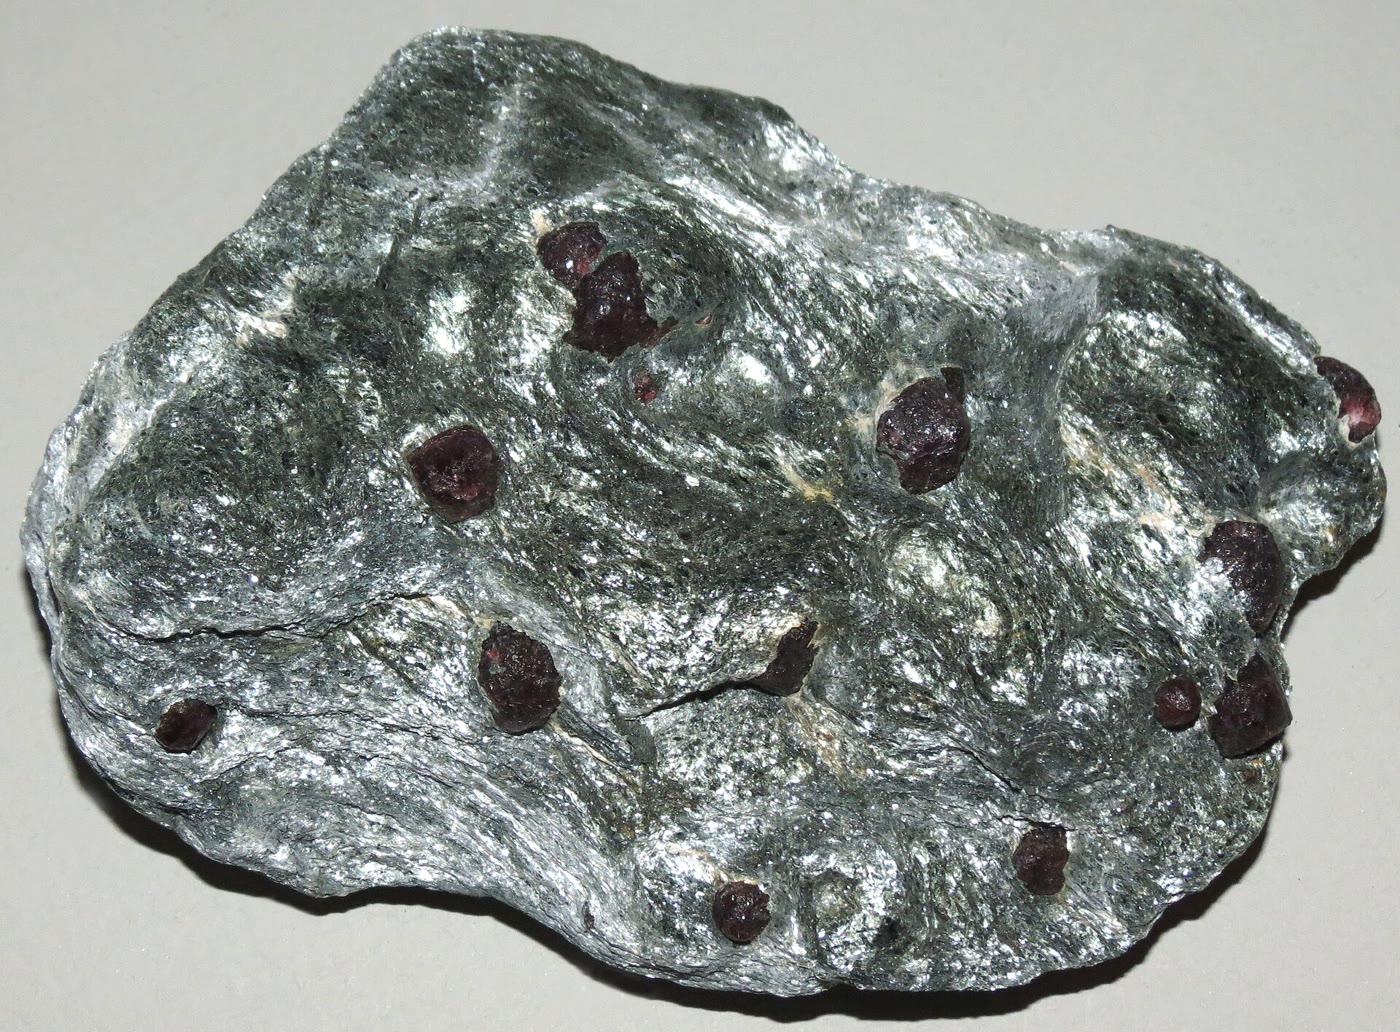
\includegraphics[width=0.62\linewidth]{images/book4/b2-11-garnet-schist.jpg}
\par\smallskip{\small Um granada-xisto: cristais de granada vermelho-escuros crescidos em uma
matriz foliada de micas. Cada granada pode guardar, do núcleo à borda, um
registro da trajetória da rocha. Fotografia de James St.~John, CC BY 2.0.}
\end{omfigure}

\section{Exercícios}

\begin{exercise}[$\star$]\label{exo:b2:pt-paths:1}
Seis amostras de uma mesma formação de lamito, coletadas ao longo de uma estrada, contêm: (A) clorita,
muscovita, quartzo; (B) biotita, clorita, muscovita, quartzo; (C) granada, biotita,
muscovita, quartzo; (D) estaurolita, granada, biotita, muscovita, quartzo; (E) cianita,
estaurolita, biotita, muscovita, quartzo; (F) silimanita, biotita, muscovita, quartzo.
(a) Em que zona barroviana fica cada uma? (b) Quantas isógradas a estrada atravessa, e
quais? (c) Por que não basta conhecer as isógradas para traçar o \omterm{def:b2:pt-paths:barrovian}{gradiente metamórfico
de campo}?
\end{exercise}
% ledger: iugs:barrow

\begin{exercise}[$\star$]\label{exo:b2:pt-paths:2}
Uma granada tem $X_{\text{Mg}} = 0.10$ e $X_{\text{Fe}} = 0.80$, a biotita ao lado dela
$X_{\text{Mg}} = 0.45$ e $X_{\text{Fe}} = 0.50$. (a) Calcule $K_D$ e $\ln K_D$.
(b) Com a calibração deste capítulo, calcule a temperatura a \qty{5}{kbar} e a
\qty{7}{kbar}. (c) O resultado é um indicador de temperatura ou de pressão?
\end{exercise}
% ledger: h97:ideal, h97:fs-reaction

\begin{exercise}[$\star$]\label{exo:b2:pt-paths:3}
Um \omterm{def:b2:metamorphic-facies:protoliths}{metapelito} dá \qty{580}{\celsius} e \qty{6.0}{kbar}. (a) Sob rochas de densidade
média \qty{2800}{kg.m^{-3}} ($g = \qty{9.81}{m.s^{-2}}$), a que profundidade ele estava? (b) Que
gradiente de temperatura isso implica a partir de \qty{10}{\celsius} na superfície? (c) A
linha experimental cianita $=$ silimanita passa por \qty{3.67}{kbar} a
\qty{500}{\celsius} e por \qty{5.77}{kbar} a \qty{600}{\celsius}: que aluminossilicato
a rocha deveria conter?
\end{exercise}
% ledger: hm93:table11

\begin{exercise}[$\star$]\label{exo:b2:pt-paths:4}
Para a \omterm{def:b2:pt-paths:ocean-floor}{serpentinização} da forsterita escrita neste capítulo: (a) verifique que a
equação está equilibrada em massa, com as massas molares 140.693 (forsterita), 18.015 (água),
277.112 (serpentina) e \qty{58.320}{g.mol^{-1}} (brucita); (b) calcule a variação de
volume dos sólidos; (c) calcule as densidades da olivina e dos produtos.
(d) O que essa variação faz a um \omterm{def:b2:mantle-melting:peridotites}{peridotito} serpentinizado sob o fundo do mar?
\end{exercise}
% ledger: rh95:serpentine

\begin{exercise}[$\star\star$]\label{exo:b2:pt-paths:5}
Calibre o termômetro a partir de quatro dos experimentos a \qty{2.07}{kbar}: $\ln K_D =
-1.157$ e $-1.255$ a \qty{799}{\celsius}, $-1.738$ e $-1.826$ a \qty{550}{\celsius}.
(a) Faça a média de cada par e encontre a reta $\ln K_D = a/T + b$ que passa pelas duas médias.
(b) Deduza $\Delta_r H$ e $\Delta_r S$, com $\Delta_r V = \qty{0.311}{J.bar^{-1}}$.
(c) Compare as temperaturas que sua calibração e a do capítulo dão a
\qty{5}{kbar} para $K_D = 0.18$, $0.10$ e $0.30$. O que você conclui sobre a
extrapolação de uma calibração?
\end{exercise}
% ledger: h97:fs-data, h97:ideal

\begin{exercise}[$\star\star$]\label{exo:b2:pt-paths:6}
(a) A partir dos volumes molares a \qty{298}{K} (almandina 115.32, piropo 113.12, anita
154.30, flogopita 149.65, grossulária 125.28, anortita 100.79, cianita 44.15, quartzo
\qty{22.69}{cm^3.mol^{-1}}), calcule o $\Delta_r V$ da troca e da reação
GASP, e compare com os valores que as calibrações usam, \num{0.311} e
\qty{-6.21}{J.bar^{-1}}. (b) Para $K_D = 0.18$, de quantos kelvin um erro de
\qty{1}{kbar} desloca a temperatura? (c) Ao longo da linha GASP de uma rocha com
$X_{\text{Ca}}/X_{\text{an}} = 0.20$, de quantos bar um erro de \qty{17}{K} desloca
a pressão?
\end{exercise}
% ledger: rh95:gb-gasp, rh95:al2sio5, h97:fs-reaction, kn88:gasp

\begin{exercise}[$\star\star$]\label{exo:b2:pt-paths:7}
A \qty{600}{\celsius}, uma granada tem $X_{\text{Ca}} = 0.08$ e o plagioclásio ao lado dela
$X_{\text{an}} = 0.30$. (a) Calcule a pressão GASP. (b) Refaça o cálculo com $X_{\text{an}} =
0.35$. (c) A que profundidade estava a rocha, para uma densidade média de \qty{2800}{kg.m^{-3}}?
\end{exercise}
% ledger: kn88:gasp

\begin{exercise}[$\star\star$]\label{exo:b2:pt-paths:8}
Use as idades da titanita das rochas subductadas mais profundas dos Alpes: cerca de \qty{3.5}{GPa} a
$35.1 \pm \qty{0.9}{Ma}$, \qty{1.0}{GPa} a $32.9 \pm \qty{0.9}{Ma}$, \qty{0.45}{GPa} a
$31.8 \pm \qty{0.5}{Ma}$. (a) Com uma densidade média de \qty{3000}{kg.m^{-3}}, converta as
pressões em profundidades. (b) Calcule as duas taxas médias de \omterm{def:b2:pt-paths:exhumation}{exumação} e compare com os
3.4 e \qty{1.6}{cm.yr^{-1}} publicados. (c) Qual é a incerteza do primeiro intervalo de
tempo, e que faixa de taxas ela admite? (d) Compare com a taxa de erosão do
modelo de espessamento, \qty{0.5}{mm.yr^{-1}}.
\end{exercise}
% ledger: rh01:exhumation

\begin{exercise}[$\star\star$]\label{exo:b2:pt-paths:9}
Para $K_D = 0.18$ a \qty{5}{kbar}, (a) calcule $\partial T/\partial\ln K_D$ e
$\partial T/\partial P$ a partir da proposição; (b) com $\sigma_{\ln K_D} = 0.05$ (um
erro de \qty{5}{\percent} em $K_D$) e $\sigma_P = \qty{1}{kbar}$, calcule $\sigma_T$.
(c) Que erro domina? Compare com a incerteza de \qty{25}{\celsius} reivindicada para
as melhores calibrações.
\end{exercise}
% ledger: h97:ideal

\begin{exercise}[$\star\star\star$]\label{exo:b2:pt-paths:10}
Uma borda de granada tem $X_{\text{Mg}} = 0.10$, $X_{\text{Fe}} = 0.75$, $X_{\text{Ca}} = 0.07$;
a biotita da matriz, $X_{\text{Mg}} = 0.42$, $X_{\text{Fe}} = 0.52$; o plagioclásio,
$X_{\text{an}} = 0.25$. (a) Aplique o método deste capítulo, partindo de \qty{6}{kbar},
até que a temperatura varie menos de \qty{1}{K}. (b) Que aluminossilicato
a rocha deveria conter (use a linha experimental do \cref{exo:b2:pt-paths:3})? (c) Por que o barômetro deve usar
o aluminossilicato realmente presente?
\end{exercise}
% ledger: h97:ideal, kn88:gasp, hm93:table11

\begin{exercise}[$\star\star\star$]\label{exo:b2:pt-paths:11}
Com $\kappa = \qty{1e-6}{m^2.s^{-1}}$: (a) calcule o tempo de relaxamento da
proposição para $L = \qty{35}{km}$ e para $L = \qty{70}{km}$. (b) O modelo erode
\qty{35}{km} em 70 milhões de anos; compare esse tempo com os dois de (a). (c) Explique,
a partir desses tempos, por que a rocha do modelo atinge seu pico térmico depois de seu pico
de pressão. (d) Se a erosão fosse dez vezes mais rápida, o que mudaria na trajetória?
\end{exercise}
% ledger: delaney:conductivity, et84:ptt

\begin{exercise}[$\star\star\star$]\label{exo:b2:pt-paths:12}
Tome uma crosta de \qty{35}{km} de espessura e densidade \qty{2800}{kg.m^{-3}} sobre um manto de
\qty{3300}{kg.m^{-3}}. (a) A que profundidade a pressão chega a \qty{28}{kbar}, o
mínimo para a coesita de Dora Maira? (b) E a \qty{40}{kbar}, para os diamantes de Kokchetav?
(c) Que gradiente médio \qty{700}{\celsius} à profundidade de (a) implica, e em que
série ele cai? (d) A \qty{3.4}{cm.yr^{-1}}, quanto tempo leva a subida da profundidade
de (a) até \qty{35}{km}?
\end{exercise}
% ledger: chopin84:coesite, ss90:diamond, rh01:exhumation

\section{Problema: a viagem de uma granada}

\begin{problem}[{Problema de fim de semana --- termobarometria, trajetória e taxa de exumação de um
xisto}]
\label{pb:b2:pt-paths:1}
Um xisto a cianita, granada e biotita contém granadas com um núcleo e uma borda. O núcleo engloba
biotita, plagioclásio e cianita; a borda toca a biotita e o plagioclásio da
matriz. Em torno das granadas, parte da cianita é substituída por silimanita, e nas bordas das
granadas cresceu um pouco de clorita. As análises são:
\begin{center}
\small
\begin{tabular}{@{}lccc@{}}
\hline
 & $X_{\text{Mg}}$ & $X_{\text{Fe}}$ & $X_{\text{Ca}}$ ou $X_{\text{an}}$\\
\hline
núcleo da granada & 0.080 & 0.760 & 0.050\\
biotita incluída no núcleo & 0.40 & 0.58 & ---\\
plagioclásio incluído no núcleo & --- & --- & 0.25\\
borda da granada & 0.120 & 0.720 & 0.060\\
biotita da matriz & 0.46 & 0.53 & ---\\
plagioclásio da matriz & --- & --- & 0.28\\
\hline
\end{tabular}
\end{center}
Use o termômetro granada--biotita e o barômetro GASP deste capítulo (mistura ideal),
$R = \qty{8.314}{J.mol^{-1}.K^{-1}}$, $g = \qty{9.81}{m.s^{-2}}$, uma densidade média de
\qty{2800}{kg.m^{-3}} acima da rocha, e arredonde cada razão a quatro casas decimais.

\noindent\textbf{Parte I --- As temperaturas.}
\begin{enumerate}
\item Calcule $X_{\text{Mg}}/X_{\text{Fe}}$ no núcleo da granada e na biotita
incluída, e depois $K_D$ e $\ln K_D$ para o núcleo.
\item Faça o mesmo para a borda e a biotita da matriz.
\item Calcule a temperatura do núcleo a \qty{6}{kbar}.
\item Calcule a temperatura da borda a \qty{6}{kbar}.
\item De quantos kelvin um erro de \qty{1}{kbar} mudaria essas temperaturas?
\item Por que o núcleo é emparelhado com a biotita incluída, e a borda com a biotita
da matriz?
\end{enumerate}

\noindent\textbf{Parte II --- As pressões.}
\begin{enumerate}[resume]
\item Calcule a pressão $P_0$ dos membros extremos da reação GASP às duas temperaturas
das questões~3 e~4.
\item Calcule a pressão GASP do núcleo à temperatura da questão~3.
\item Calcule a pressão GASP da borda à temperatura da questão~4.
\item Recalcule a temperatura da borda à pressão da questão~9, depois sua
pressão a essa temperatura, e mais uma vez a temperatura. Dê a temperatura e a
pressão da borda.
\item Faça o mesmo uma vez para o núcleo. Por que ele muda tão pouco?
\item Converta as pressões do núcleo e da borda em profundidades.
\item A linha experimental cianita $=$ silimanita passa por 3.67, 5.77 e
\qty{7.86}{kbar} a 500, 600 e \qty{700}{\celsius}. Que aluminossilicato era estável
quando o núcleo cresceu, e quando a borda cresceu? A cianita do núcleo é coerente?
\end{enumerate}

\noindent\textbf{Parte III --- A trajetória.}
\begin{enumerate}[resume]
\item Entre o núcleo e a borda, de quanto variaram a temperatura e a pressão?
A granada crescia na \omterm{def:b2:pt-paths:paths}{trajetória progressiva} ou na retrógrada?
\item A silimanita substitui a cianita em torno das granadas. À temperatura da borda,
abaixo de que pressão a rocha deve ter passado para que isso aconteça? O que a rocha fez
depois que a borda cresceu?
\item A clorita cresce nas bordas das granadas. Que parte da trajetória ela registra?
\item Desenhe a trajetória: núcleo, borda, silimanita, clorita. Ela é horária ou anti-horária?
Que pico veio primeiro?
\item O modelo de espessamento deste capítulo leva sua rocha a um pico térmico de
\qty{593}{\celsius} a \qty{7.8}{kbar}. A trajetória do xisto é do mesmo tipo?
\end{enumerate}

\noindent\textbf{Parte IV --- Com que rapidez.}
\begin{enumerate}[resume]
\item A borda da granada dá uma idade samário--neodímio de $412.0 \pm \qty{1.5}{Ma}$, tomada
como a idade do pico; uma muscovita da matriz dá uma idade argônio de $398.0 \pm
\qty{1.0}{Ma}$, o momento em que a rocha se resfriou abaixo de \qty{405}{\celsius}. Calcule
a taxa média de resfriamento entre as duas.
\item A temperatura de fechamento de \qty{405}{\celsius} supõe um resfriamento a
\qty{10}{\celsius} por milhão de anos. A taxa da questão~19 pede um valor mais alto ou
mais baixo, e por quê?
\item A \qty{398}{Ma}, tome uma geoterma de \qty{30}{\celsius\per\km} a partir de
\qty{10}{\celsius} na superfície. A que profundidade a muscovita se fechou?
\item Quanto a rocha subiu entre o pico e o fechamento da muscovita?
\item Qual é a incerteza do intervalo de tempo?
\item Calcule a taxa média de \omterm{def:b2:pt-paths:exhumation}{exumação} do pico ao fechamento da muscovita, em
milímetros por ano e arredondada ao décimo: o número-chave deste problema.
\end{enumerate}
\end{problem}
% ledger: h97:ideal, h97:fs-reaction, kn88:gasp, hm93:table11, h09:muscovite, scmr:ptt, et84:ptt
